
\section{Numerical Experiment}
\subsection{Introduction}
\begin{frame}
  \frametitle{Implementation and Dataset}
  All the described algorithms have been implemented in \alert{C++}.
  {\small Code:~\url{https://github.com/arn4/colloquio/tree/main/rbm-library}}
  \vspace{10pt}
  
  \begin{columns}[T]
    \column{0.8\textwidth}
      \onslide<2->{
        Dataset: \alert{MNIST} for handwritten digit recognition. \(28\times28\) pixels, B\&W images of digits from 0 to 9.
        \begin{itemize}
          \item \structure{training set}: \(60'000\) images. 
                Divided in 5421 batches containing a single rep per class.
                Only \(54'210\) used for training (90\%).
          \item \structure{test set}: \(10'000\) images, with labels.
        \end{itemize}
      }
      \onslide<3->{
        RBM:
        \begin{itemize}
          \item 784 visible units; 500 hidden
          \item learning rate, weight decay and momentum are the same in every training to better compare algorithms.
        \end{itemize}
        All algorithms run for 50 epochs.
      }
    \column<2->{0.2\textwidth}
      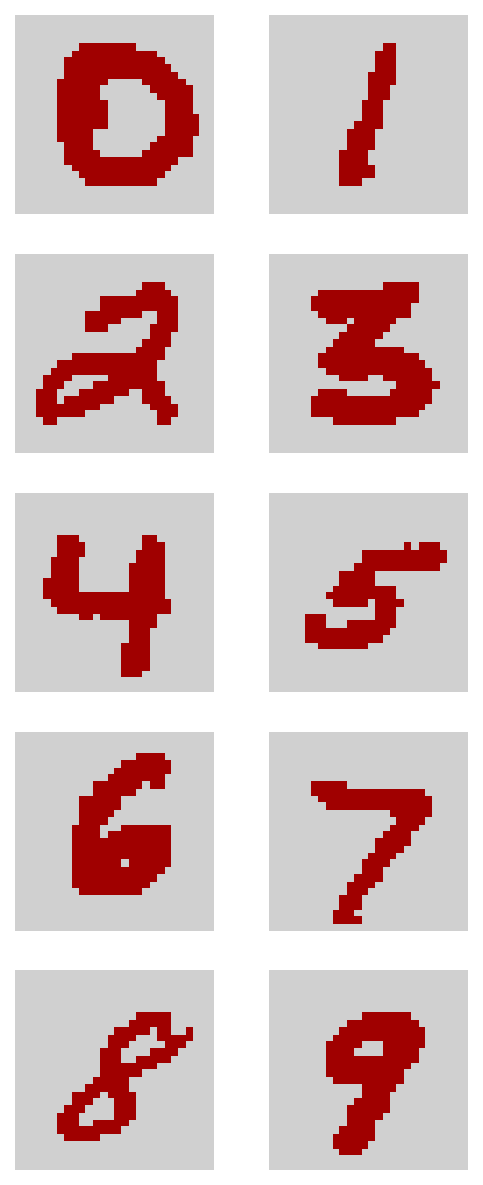
\includegraphics[width=0.8\textwidth]{img/mnist-example.pdf}
  \end{columns}
\end{frame}

%%%%%%%%%%%%%%%%%%%%%%%%%%%%%%%%%%%%%%%%%%%%%%%%%%%%%%%%%%%%%%%%%%%%%%%%%%%%%%%%%%%%%%%%%%%%%%%%%%%%

\subsection{Results}
\begin{frame}
  \frametitle{Pseudo-likelihood}
  \begin{columns}
    \column{0.51\textwidth}
      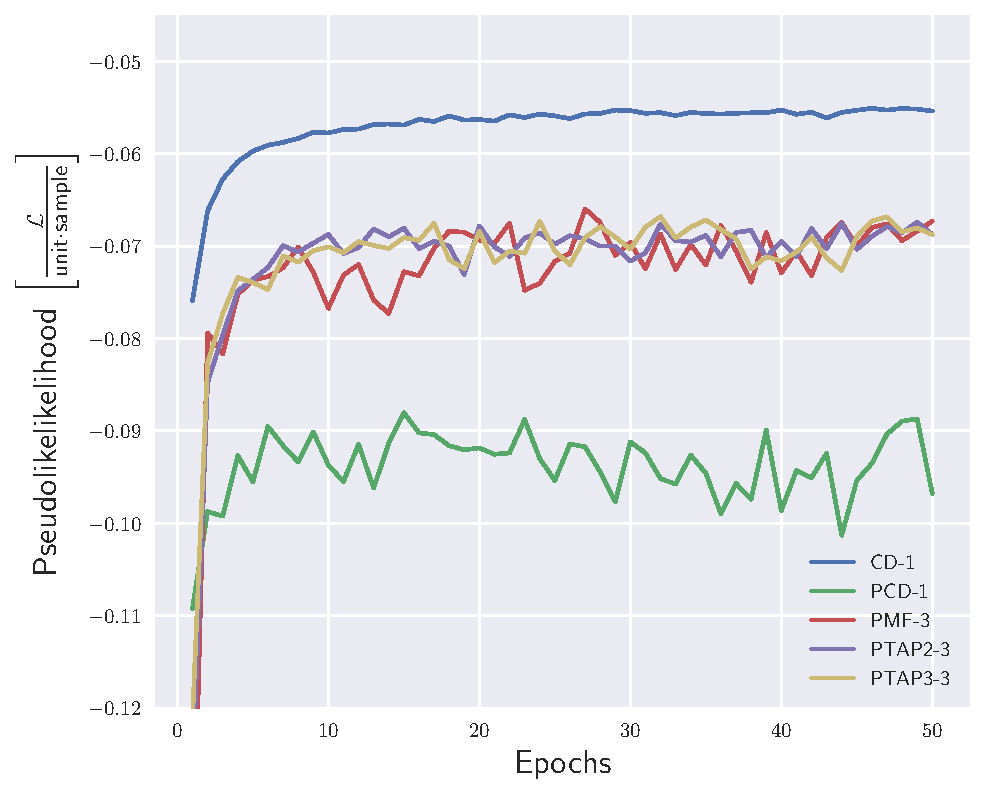
\includegraphics[width=\textwidth]{img/numerical-experiments/psl-plot-global.pdf}
    \column{0.51\textwidth}
      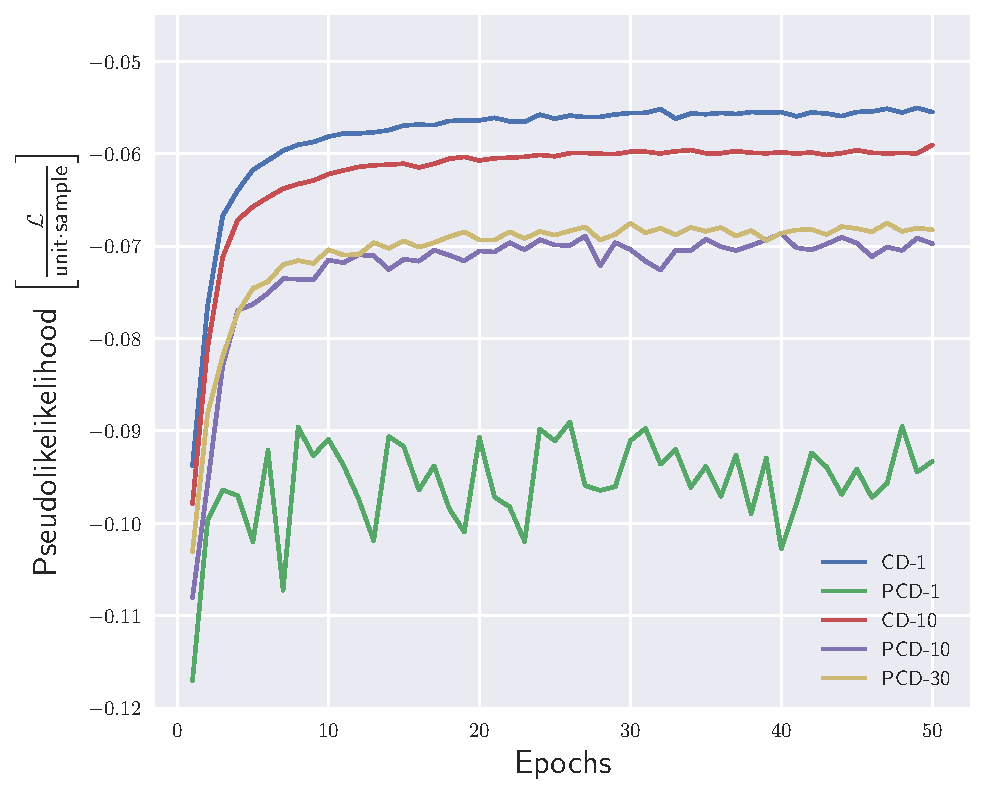
\includegraphics[width=\linewidth]{img/numerical-experiments/psl-plot-classical.pdf}
  \end{columns}
\end{frame}

\begin{frame}
  \frametitle{Stability test}
  \begin{columns}
    \column{0.45\textwidth}
      \centering
      \structure{CD-1}
      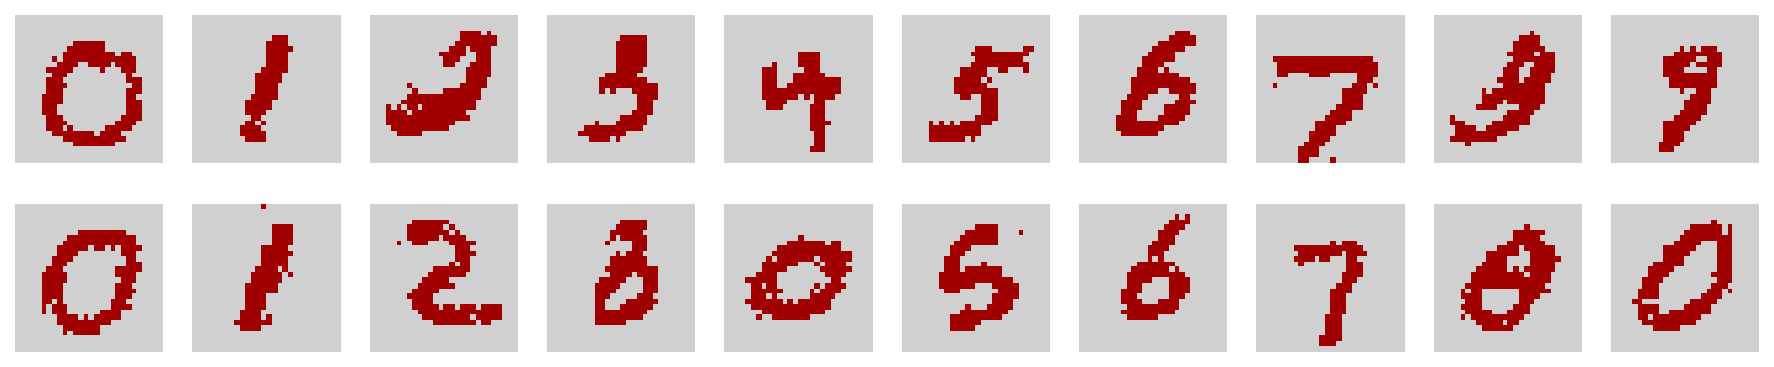
\includegraphics[width=\textwidth]{img/numerical-experiments/stability-cd-1.pdf}
    \column{0.45\textwidth}
    \centering
      \structure{PCD-1}
      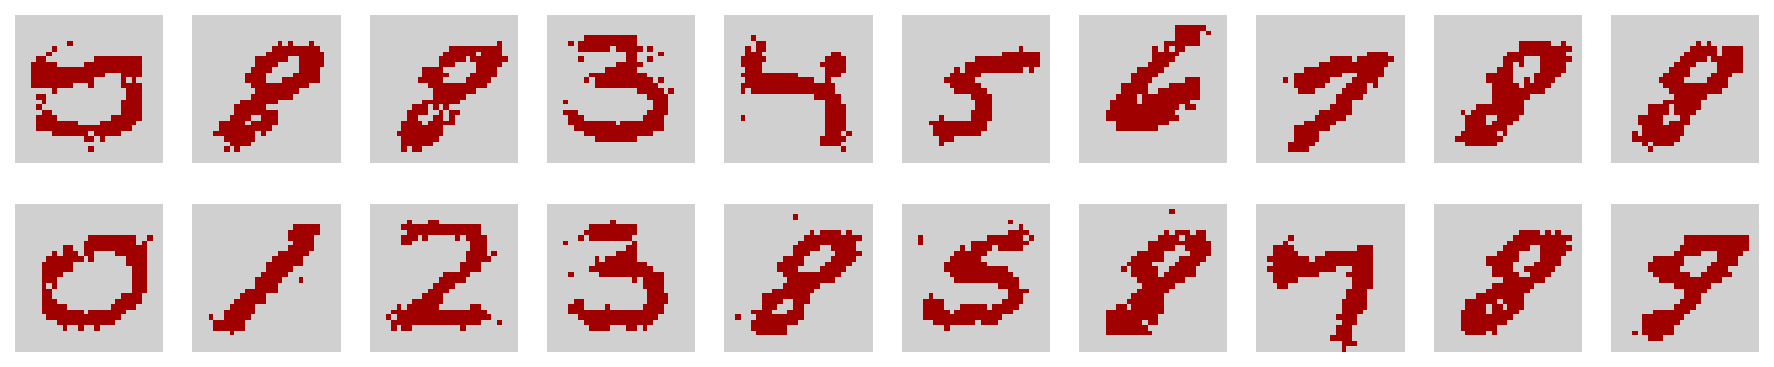
\includegraphics[width=\linewidth]{img/numerical-experiments/stability-pcd-1.pdf}
  \end{columns}
  \vspace{5pt}
  \begin{columns}
    \column{0.45\textwidth}
    \centering
    \structure{MF-3}
    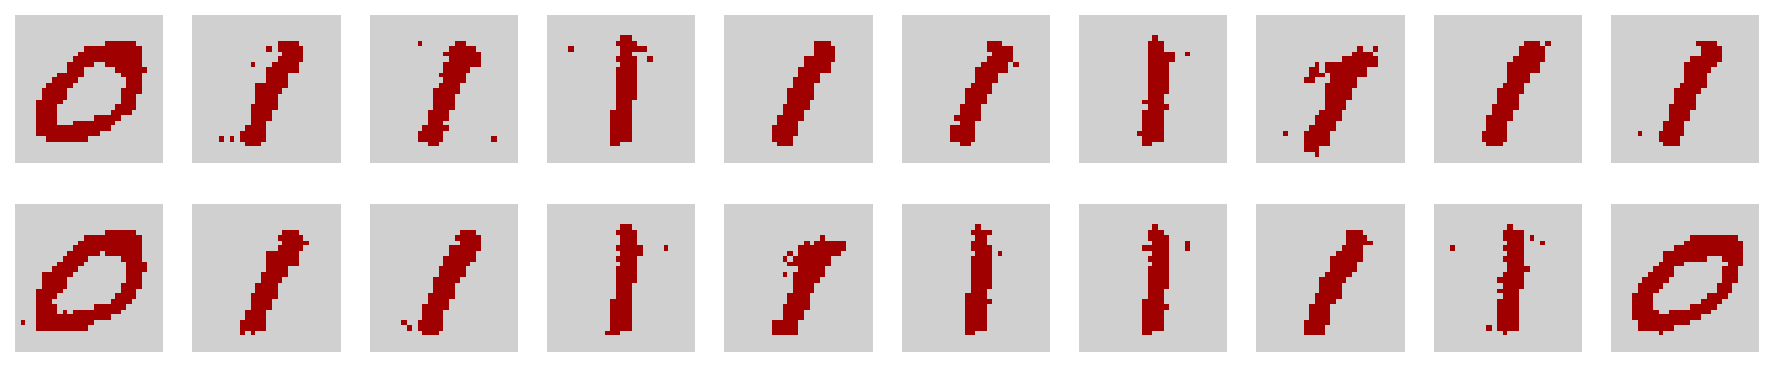
\includegraphics[width=\textwidth]{img/numerical-experiments/stability-mf-3.pdf}
    \column{0.45\textwidth}
    \centering
    \structure{PMF-3}
    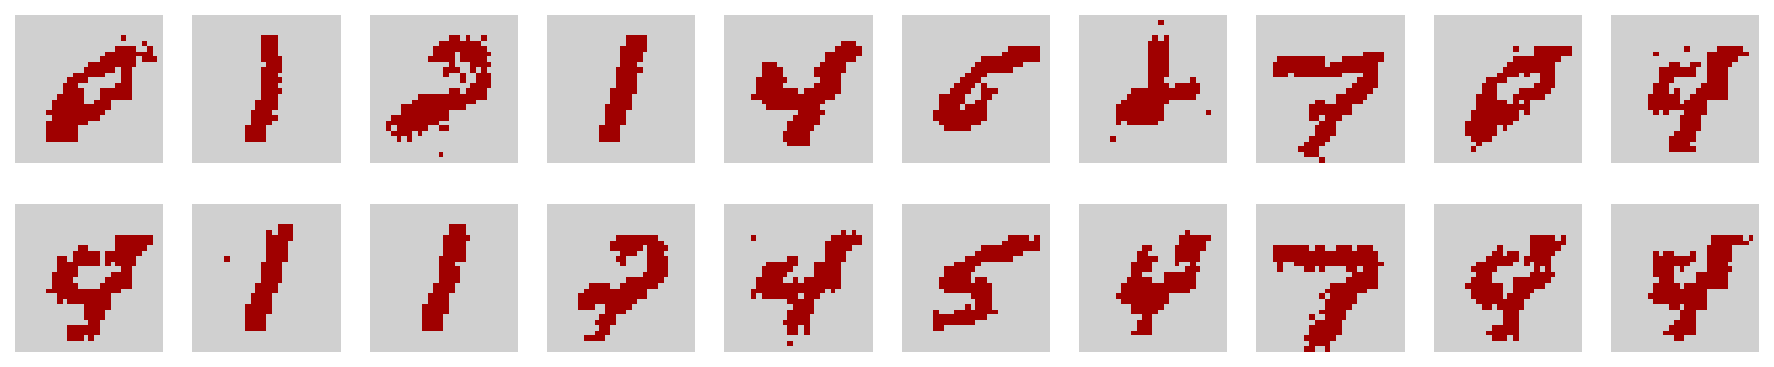
\includegraphics[width=\linewidth]{img/numerical-experiments/stability-pmf-3.pdf}
  \end{columns}
  \vspace{5pt}
  \begin{columns}
    \column{0.45\textwidth}
    \centering
    \structure{TAP2-3}
    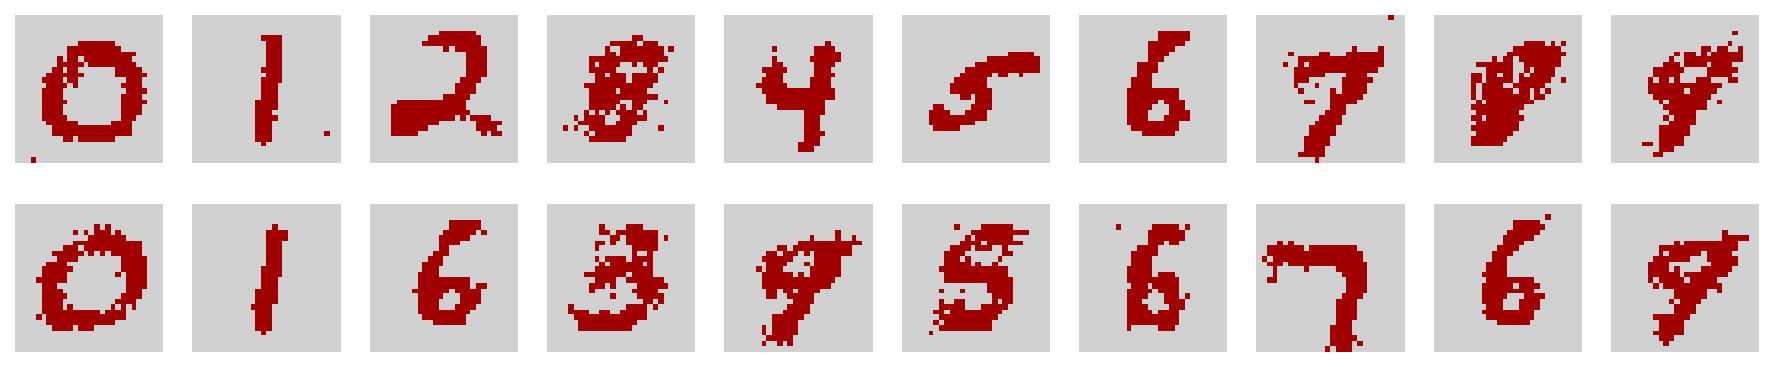
\includegraphics[width=\textwidth]{img/numerical-experiments/stability-tap2-3.pdf}
    \column{0.45\textwidth}
    \centering
    \structure{PTAP2-3}
    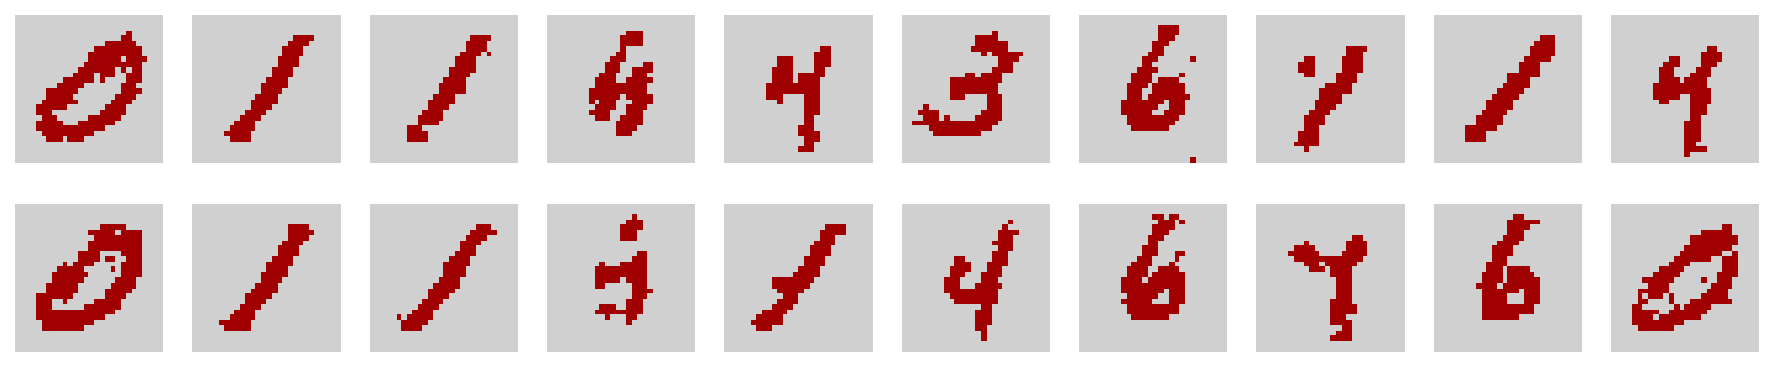
\includegraphics[width=\linewidth]{img/numerical-experiments/stability-ptap2-3.pdf}
  \end{columns}
  \vspace{5pt}
  \begin{columns}
    \column{0.45\textwidth}
    \centering
    \structure{TAP3-3}
    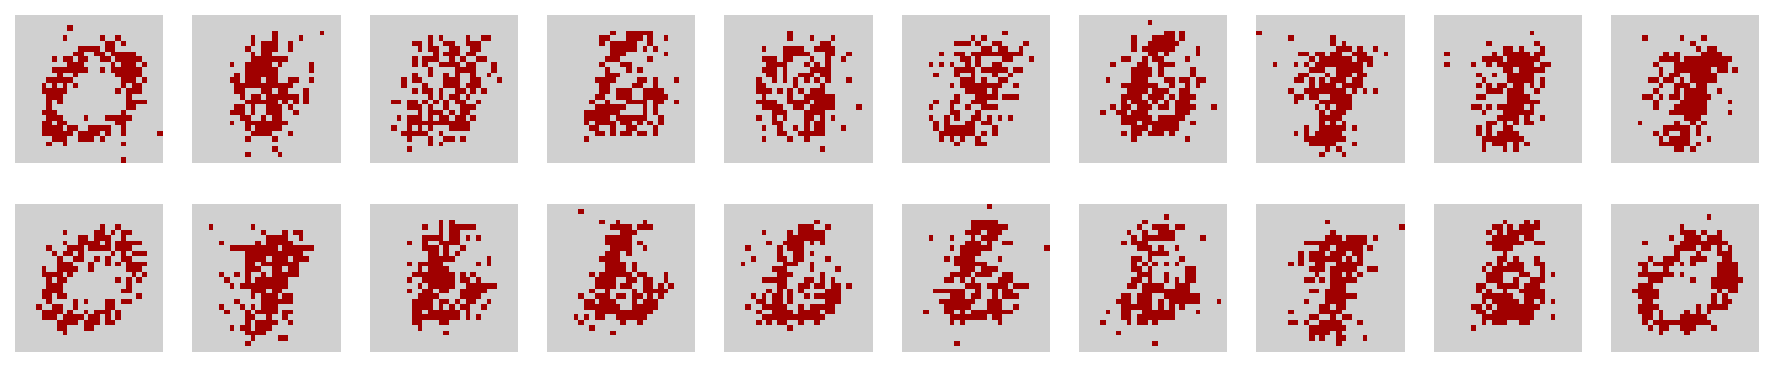
\includegraphics[width=\textwidth]{img/numerical-experiments/stability-tap3-3.pdf}
    \column{0.45\textwidth}
    \centering
    \structure{PTAP3-3}
    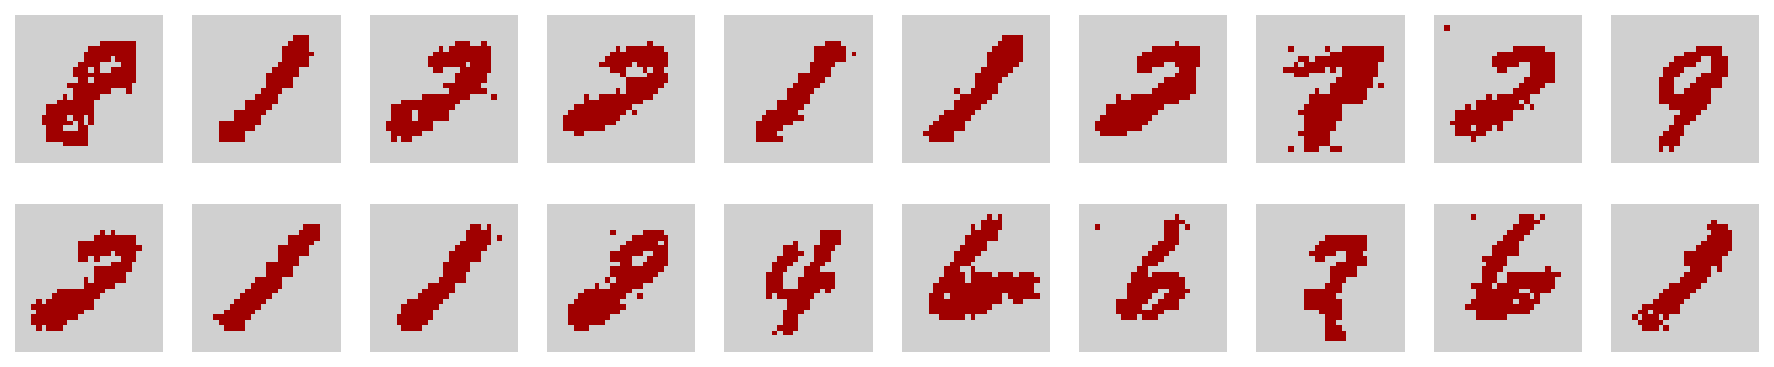
\includegraphics[width=\linewidth]{img/numerical-experiments/stability-ptap3-3.pdf}
  \end{columns}
\end{frame}

\begin{frame}
  \frametitle{Classification}
  \begin{columns}
    \column{0.4\textwidth}
       \alert{Logistic classifier} run over the activation probabilities of the hidden layer.\\
        Regression on pure images scored 91.82\% accuracy on the test set.
    \column{0.6\textwidth}
      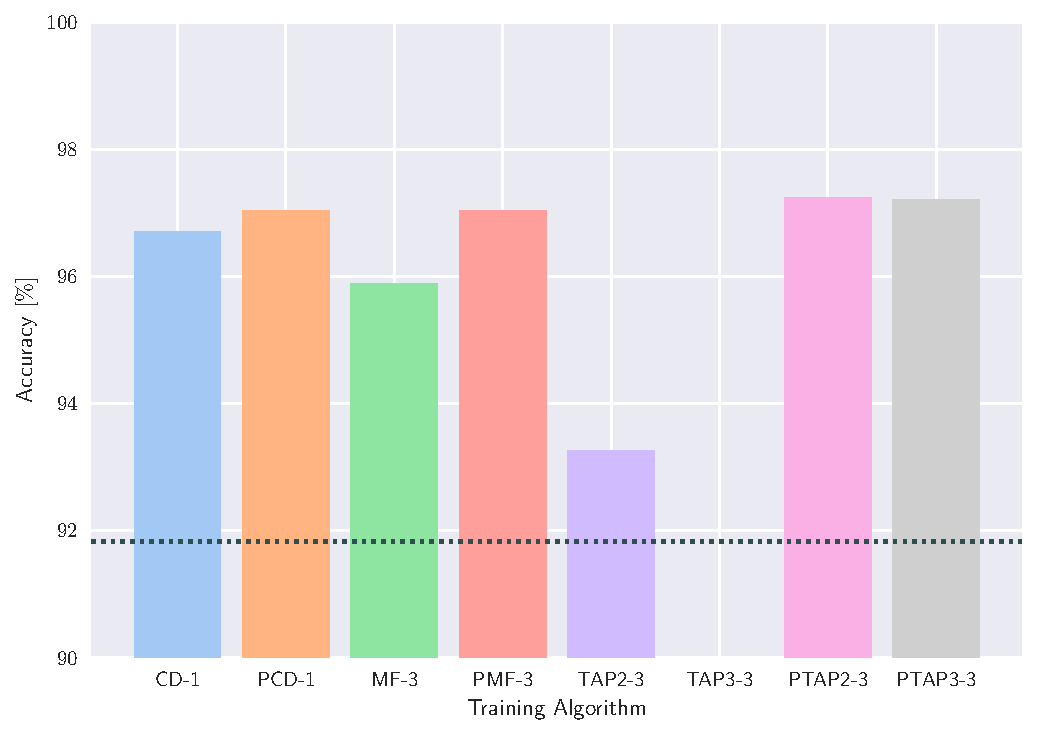
\includegraphics[width=\linewidth]{img/numerical-experiments/acc-hist.pdf}
  \end{columns}
\end{frame}

%%%%%%%%%%%%%%%%%%%%%%%%%%%%%%%%%%%%%%%%%%%%%%%%%%%%%%%%%%%%%%%%%%%%%%%%%%%%%%%%%%%%%%%%%%%%%%%%%%%%

\begin{frame}
  \frametitle{Conclusions}
  \begin{itemize}[<+->]
    \item Pseudo-likelihood is not the best quantity for monitor learning.\\
    \emph{Visible vector free energy} could be a better alternative
    \item \structure{TAP2} and \structure{TAP3} are not behaving as expected. Probably weight decay is
          too low and high-temperature hypothesis does not hold throughout learning. Persistent versions are clearly better
    \item \structure{PCD-1}, \structure{PMF-3}, \structure{PTAP2-3}, and \structure{PTAP3-3} perform similarly probably because the theoretical limit of maximum likelihood is close.\\
          \structure{PCD-30} scores 97.7\%. \\
          Algorithms should be compared on ``more difficult''  dataset.
  \end{itemize}
\end{frame}

